%Vorlage fuer Thesen an der FFHS
\documentclass{ffhsthesis}

\usepackage[utf8]{inputenc}
\usepackage[style=ieee,backend=biber]{biblatex}
\usepackage{bashful}

% Literaturverzeichnis
\addbibresource{lib/literatur.bib}

% "\ToDo"-Befehl in rotem Text
\newcommand*{\ToDo}[1]{\textcolor{red}{TODO: #1}}

% TOC mit Hyperlinks %
\usepackage{hyperref}
\hypersetup{
    colorlinks,
    citecolor=black,
    filecolor=black,
    linkcolor=black,
    urlcolor=black
}

\begin{document}

\dokumentTyp{Seminararbeit}
\studiengang{INF}
\title{simple web file transfer}
%\title{FileTransfer: Analyse und Vergleich HTTP(s)-Lösung mit FTP}
%\subtitle{auf einem Synology NAS DS215+} % optional
%\titelbild[height=2cm,width=10cm]{ffhslogo}  % optional
\author{Adriano Hänggli}
% \date{}
\wohnort{Brugg}
%\referent{Name des Referenten\\ Titel\\Unterrichtetes Fach}
\referent{Prof. Dr. Heinrich Zimmermann\\ Dozent für\\Seminararbeit}
\eingereichtBei{Dr.\ Oliver Kamin\\Departement Informatik\\Departementsleiter} 

% \dedication{Diese Thesis widme ich\\\dots}

\maketitle

% Abstract/Zusammenfassung
\begin{zusammenfassung}
    ... Deutsche Zusammenfassung ...
\end{zusammenfassung}
    
\begin{abstract}
    ... English summary ...
\end{abstract}

\tableofcontents


% Abkürzungen
\begin{abkuerzungen}[MUSTER] % Das Muster dient zur Bestimmung der Einrueckungstiefe
    \item[DInf] Departement Informatik
    \item[FFHS] Fernfachhochschule Schweiz
\end{abkuerzungen}

% Glossar
\begin{glossar}[Prioritätenskala] % Das Muster dient zur Bestimmung der Einrueckungstiefe
    \item[DInf]             Departement Informatik
    \item[FFHS]             Fernfachhochschule Schweiz
    %\item[Prioritätenskala] Die Prioritätenskala ist innerhalb des Projektes stets mit MUSS, SOLL, KANN gekennzeichnet. Dabei gilt die hier definierte ordinale Rangfolge.
	%\item[Client]           Gemeint ist jeweils das Front-End. Mit Front-End sind innerhalb dieses Projektes alle Teile gemeint, die primär für die Darstellung, Ausgabe sowie Eingabe von Daten über das GUI genutzt werden.
    %\item[Server]           Gemeint ist jeweils das Back-End. Damit sind alle Teile gemeint, die über den NodeJS-Server und nicht direkt im Browser der Benutzers laufen.
    %\item[GUI]              Grafische Benutzeroberfläche, Benutzerschnittstelle der Applikation
    %\item[MVP]              Ein Minimum Viable Product (MVP), ist die erste minimal funktionsfähige Iteration eines Produkts, das entwickelt werden muss, um mit minimalem Aufwand den Kunden-, Markt- oder Funktionsbedarf zu decken und handlungsrelevantes Feedback zu gewährleisten.
    %\item[PaaS]             Platform as a Service
\end{glossar}




\startThesis % Befehl muss vor dem ersten chapter stehen (Seitennummerierung!)
\chapter{Einleitung}
Im folgenden Kapitel werden Motivation und Problemstellung mit dem Praxisbezug erläutert. 
Dabei wird aus Gründen der besseren Lesbarkeit ausschliesslich 
die männliche Form benutzt. Es können dabei aber sowohl männliche, 
weibliche als auch non-binäre Personen gemeint sein.

\section{Ausgangslage}
Software altert nicht direkt, kann aber nach einiger Zeit eingeschränkter Wartung - oder noch schlimmer: komplett ohne Wartung - in die Jahre kommen. 
So kann - nebst gesetzlicher Änderungen, Fusionen oder Softwarezwang - das Bedürfnis entstehen, eine Software mit einer zeitgemässen Lösung auszuwechseln.   

Dieser Trend zeichnet sich derzeit schweizweit im Bereich der Gemeinden, Städte und Energieversorgungsunternehmen 
(nachfolgend ``Kunden'' genannt) ab. 
Kleinere Gemeinden und EVU fusionieren um ihre Ressourcen zu bündeln und die Administration zu vereinfachen. 
Mittlere und Grössere Kunden suchen alternative Lösungen um mit den Gesetzesänderungen und den Marktbegleitern mitzuhalten.  

Die teilweise über mehrere Jahrzehnte erfassten Datenbestände müssen dann in die neue Software übernommen werden. 
Ein Start auf grüner Wiese kommt im Umfeld der Öffentlichen Verwaltung sowie der Energiebranche fast nie in Frage. 
Zu wichtig sind die bestehenden Informationen für Auskünfte und Prognosen. 
Über die Jahre sammelt sich daher eine Unmenge an Daten: 
Von weniger heiklen Zählerständen bis hin zu spannenden Umzugsdaten und äusserst geheim zu haltenden Steuerdeklarationen. 

Um die Daten aus der alten Software zu übernehmen, müssen diese an einen Migrator übermittelt werden. 
Für die Datenübermittelung gibt es in der Schweiz keinen einheitlichen Standard. 
Es existieren folglich bereits unzählige Möglichkeiten.
E-Mail, CloudDienste (OneDrive, Dropbox, usw.) sowie FTP sind nur einige davon. E-Mail und CloudDienste fallen sehr oft weg, da sie - im Falle von Steuerdaten, die in allen Fällen in der Schweiz bleiben müssen - gesetzlich nicht erlaubt sind oder aber die Datenmenge einfach zu gross ist. 
Die häufigste Übermittlungsart im Umfeld des Autors ist folglich FTP. 

\section{Problemstellung}
Die Nutzung von FTP bedarf eines Happens an Informatik-Kenntnissen. Das stellt gerade bei kleinen Kunden ein Problem dar.
Oft ist die Informatik bei den Finanzen oder der Administration eingebunden. 
Leider weisen die dort zuständigen Personen oft alles andere als eine nützliche Affinität zur IT auf. 
Erste Unterstützungsarbeiten entstehen somit bereits bevor mit der Migration begonnen werden kann. 
(Rein persönliche Sicht des Autors deren Wahrheitsgehalt bislang nicht statisch erhoben wurde)
Ein weitere Herausforderung entsteht dadurch, dass zwischen Migrator und Kunden sehr häufig noch Vertriebspartner stehen. 
Diese können Aufträge mehrerer Kunden beim selben Migrator platzieren. 
Die Mitarbeiter des Vertriebspartners sollten beim Migrator keinen unfreiwilligen Einblick über andere laufende Projekte erhalten. 
Technisch müssen daher derzeit mehrere FTP-Accounts herhalten. Es entsteht erheblicher administrativer Aufwand um die FTP-Accounts zu verwalten.

Ein weiteres Problem entsteht durch das Rücksenden der Daten. 
Die migrierten Daten müssten im Format der neuen Software irgendwie im System des Kunden landen.
Dafür müssen die Daten wieder zurückgesendet werden. Gerade bei grossen Kunden oder Kunden mit kantonalen Mutterkonzernen sind FTP-Verbindungen - bzw. generell eingehenden Verbindungen - gesperrt. 
Offen hingegen sind meist SSL verschlüsselte Webseiten. 
Es bietet sich daher an, anstelle von FTP die Datenübermittelung mittels einer HTTPS-Website vorzunehmen. 
Um zu entscheiden solch eine Umstellung im geschäftlichen Umfeld sinnvoll ist, müssen folgende zentrale Fragen beantwortet werden:
\textit{Wie verhält sich die Performanz beim Datenaustausch via HTTPS?} 
\textit{Wie einfach ist der Umgang mit einer Dateiübertragung via Web?}

Diese Fragen werden mittels Prototyp einer Web-Applikation beantwortet. 
Es bestehen bereits viele Programme für den Datenaustausch via Web. Oft sind diese aber bei grossen Cloud-Anbietern gehostet. 
Die recherchierten Selfhosted-Lösungen beinhalten alle wiederum eine administrativ Aufwändige Erfassung von Nutzer-Accounts oder aber machen die Daten generell öffentlich zugänglich.

\section{Aufbau}
Die Seminararbeit ist in drei Teile gegliedert. 
Der erste Teil besteht aus der Spezifikation des Prototyps. 
%Darstellung des Stand des Wissens und der Technik (bezogen auf die Problemstellung)
%Umriss des geplanten eigenen innovativen Beitrages (mit Benennung der Idee und Zielsetzungen)
%Planung des Entwicklungsvorhabens (Konzeption und Realisierungsansatz)
Im zweiten Teil wird die Realisierung dokumentiert. Der letzte Teil widmet sich der Analyse der Performanz und Rückmeldungen.
%Dokumentation der Durchführung der Entwicklung
%Dokumentation der Ergebnisse

\section{Abgrenzung}
Der Hauptinhalt der Seminararbeit bezieht sich auf das Entwickeln einer einfach bedienbaren Web-Applikation für die Datenübermittelung und Analyse der Performanz.
Die Web-Applikation muss auf einem Synology NAS DS1819+ lauffähig sein.
Die Arbeit hat nicht den Anspruch auf besondere Effizienz der Applikation, Vollständigkeit aller erdenglichen Analysen oder erhöhte Sicherheit bei der Übermittlung. 

\section{Ziele der Seminararbeit}
Die Resultate der Arbeit bilden die Grundlage dafür, ob ein Wechsel weg von FTP-Übermittlungen hin zu HTTPS weiterverfolgt werden soll beim Arbeitgeber des Autors.
Wird während der Analysen eine Tendenz zur Weiterverfolgung erkannt, soll weiter eine Schätzung über den zu erwarteten Aufwand abgegeben werden können, bis der Prototyp einsatzbereit wäre.
Im Falle einer eher negativen Tendenz beschränkt sich das Ziel auf die Auswertung der Performanz.
\chapter{Material}


\chapter{Methoden}
\chapter{Ausblick}
In Zukunft wird das in dieser Arbeit erstellte Konzept zu Testzwecken produktiv bei 100
IoT-Geräten eingesetzt. Die Evaluierung der Datenpunkte ist dabei noch nicht abgeschlossen
aber im Gange. Dabei werden die neuen Datenkorrelationen im Team diskutiert
und bewertet, die nach Abschluss dieses Verfahrens in die Firmware eingebaut
werden. Die Auswertung erfolgt dann in etwa drei Monaten nach der Aktualisierung. Dies
garantiert eine aussagekräftige Anzahl an Daten.
Um die Analysemöglichkeiten noch verbessern zu können, wird ausserdem MQTT als
neues Verbindungsprotokoll eingesetzt. Dieses Protokoll ermöglicht eine nahezu Realtime-
Analyse der gesammelten Daten, was eine geringere Reaktionszeit zur Folge hat. Diese
Strategie wird noch durch automatisierte Aktionen ergänzt, was den Arbeitsaufwand für
die Analyse minimal hält. Aus betrieblichen und datenschutzrechtlichen Gründen kann
die Strategie aber an dieser Stelle nicht näher ausgeführt werden.

\chapter{Reflexion}
Es handelt sich hierbei um meine erste wissenschaftliche Arbeit. 
Entsprechend musste ich mich vor Beginn stark in die Thematik einlesen. Dazu habe ich auch einige Beispielarbeiten gelesen.
Dies hat einiges an Zeit gekostet, wodurch ich mich viel zu spät damit auseinander gesetzt habe, 
über welches Thema ich schreiben soll. Das Coaching durch den Dozenten war daher sehr hilfreich. 
Während der Recherche zur dahinterliegenden Technologie der Arbeit, war es schwierig geeignete Quellen zu finden.
Die Themen werden in den Sachbüchern jeweils nur angeschnitten oder auf einem sehr hohen Expertenlevel sehr detailliert behandelt.
Das von mir gewünschte Mittelmass scheint leider nicht sehr weit verbreitet zu sein.
Dies kann an meiner Problemstellung zusammenliegen. Die zwar individuelle Lösung hat sehr allgemeingültige Grundlagen dahinter.
Netzwerke und deren Aufbau sind nicht gerade meine Stärke. 
Dennoch war es sehr interessant die Hintergründe dazu bei der Implementierung des Prototyps zu berücksichtigen.
\\
Ich bin froh darüber, dass es sich hierbei um eine erste wissenschaftliche Arbeit und keine Abschlussarbeit oder gar Bachelorarbeit handelt.
Mit den neu gewonnen Erfahrungen würde ich dort die Vorbereitungen und Recherche anders gestalten. 
Wäre mir von Beginn des Moduls an, ein Thema im Kopf gewesen, hätte ich die Arbeit wohl anders aufgebaut. 
Eine sinnvolle und möglichst vollständige Argumentation mit rotem Faden aufzubauen ist eine Herausforderung. 
Eventuell wäre es einfacher geworden, wenn die Fragestellung konkreter definiert worden wäre. 
Sie lässt eigentlich offen, ob der Prototyp nur ein Mittel zum Zweck oder aber der Entwurf dessen das Hauptziel ist. 
\\
Nichtsdestotrotz konnte an dieser Arbeit einiges an Erfahrung gewonnen werden. Mit den Resultaten bin ich im grossen und ganzen sehr zufrieden.
Bei der noch folgenden Bachelorarbeit werde ich jedoch die obigen Punkte verbessern. Besonders was die Definition der Fragestellung betrifft.


\chapter{Einleitung}
Im folgenden Kapitel werden Motivation und Problemstellung mit dem Praxisbezug erläutert. 
Dabei wird aus Gründen der besseren Lesbarkeit ausschliesslich 
die männliche Form benutzt. Es können dabei aber sowohl männliche, 
weibliche als auch non-binäre Personen gemeint sein.

\section{Ausgangslage}
Software altert nicht direkt, kann aber nach einiger Zeit eingeschränkter Wartung - oder noch schlimmer: komplett ohne Wartung - in die Jahre kommen. 
So kann - nebst gesetzlicher Änderungen, Fusionen oder Softwarezwang - das Bedürfnis entstehen, eine Software mit einer zeitgemässen Lösung auszuwechseln.   

Dieser Trend zeichnet sich derzeit schweizweit im Bereich der Gemeinden, Städte und Energieversorgungsunternehmen 
(nachfolgend ``Kunden'' genannt) ab. 
Kleinere Gemeinden und EVU fusionieren um ihre Ressourcen zu bündeln und die Administration zu vereinfachen. 
Mittlere und Grössere Kunden suchen alternative Lösungen um mit den Gesetzesänderungen und den Marktbegleitern mitzuhalten.  

Die teilweise über mehrere Jahrzehnte erfassten Datenbestände müssen dann in die neue Software übernommen werden. 
Ein Start auf grüner Wiese kommt im Umfeld der Öffentlichen Verwaltung sowie der Energiebranche fast nie in Frage. 
Zu wichtig sind die bestehenden Informationen für Auskünfte und Prognosen. 
Über die Jahre sammelt sich daher eine Unmenge an Daten: 
Von weniger heiklen Zählerständen bis hin zu spannenden Umzugsdaten und äusserst geheim zu haltenden Steuerdeklarationen. 

Um die Daten aus der alten Software zu übernehmen, müssen diese an einen Migrator übermittelt werden. 
Für die Datenübermittelung gibt es in der Schweiz keinen einheitlichen Standard. 
Es existieren folglich bereits unzählige Möglichkeiten.
E-Mail, CloudDienste (OneDrive, Dropbox, usw.) sowie FTP sind nur einige davon. E-Mail und CloudDienste fallen sehr oft weg, da sie - im Falle von Steuerdaten, die in allen Fällen in der Schweiz bleiben müssen - gesetzlich nicht erlaubt sind oder aber die Datenmenge einfach zu gross ist. 
Die häufigste Übermittlungsart im Umfeld des Autors ist folglich FTP. 

\section{Problemstellung}
Die Nutzung von FTP bedarf eines Happens an Informatik-Kenntnissen. Das stellt gerade bei kleinen Kunden ein Problem dar.
Oft ist die Informatik bei den Finanzen oder der Administration eingebunden. 
Leider weisen die dort zuständigen Personen oft alles andere als eine nützliche Affinität zur IT auf. 
Erste Unterstützungsarbeiten entstehen somit bereits bevor mit der Migration begonnen werden kann. 
(Rein persönliche Sicht des Autors deren Wahrheitsgehalt bislang nicht statisch erhoben wurde)
Ein weitere Herausforderung entsteht dadurch, dass zwischen Migrator und Kunden sehr häufig noch Vertriebspartner stehen. 
Diese können Aufträge mehrerer Kunden beim selben Migrator platzieren. 
Die Mitarbeiter des Vertriebspartners sollten beim Migrator keinen unfreiwilligen Einblick über andere laufende Projekte erhalten. 
Technisch müssen daher derzeit mehrere FTP-Accounts herhalten. Es entsteht erheblicher administrativer Aufwand um die FTP-Accounts zu verwalten.

Ein weiteres Problem entsteht durch das Rücksenden der Daten. 
Die migrierten Daten müssten im Format der neuen Software irgendwie im System des Kunden landen.
Dafür müssen die Daten wieder zurückgesendet werden. Gerade bei grossen Kunden oder Kunden mit kantonalen Mutterkonzernen sind FTP-Verbindungen - bzw. generell eingehenden Verbindungen - gesperrt. 
Offen hingegen sind meist SSL verschlüsselte Webseiten. 
Es bietet sich daher an, anstelle von FTP die Datenübermittelung mittels einer HTTPS-Website vorzunehmen. 
Um zu entscheiden solch eine Umstellung im geschäftlichen Umfeld sinnvoll ist, müssen folgende zentrale Fragen beantwortet werden:
\textit{Wie verhält sich die Performanz beim Datenaustausch via HTTPS?} 
\textit{Wie einfach ist der Umgang mit einer Dateiübertragung via Web?}

Diese Fragen werden mittels Prototyp einer Web-Applikation beantwortet. 
Es bestehen bereits viele Programme für den Datenaustausch via Web. Oft sind diese aber bei grossen Cloud-Anbietern gehostet. 
Die recherchierten Selfhosted-Lösungen beinhalten alle wiederum eine administrativ Aufwändige Erfassung von Nutzer-Accounts oder aber machen die Daten generell öffentlich zugänglich.

\section{Aufbau}
Die Seminararbeit ist in drei Teile gegliedert. 
Der erste Teil besteht aus der Spezifikation des Prototyps. 
%Darstellung des Stand des Wissens und der Technik (bezogen auf die Problemstellung)
%Umriss des geplanten eigenen innovativen Beitrages (mit Benennung der Idee und Zielsetzungen)
%Planung des Entwicklungsvorhabens (Konzeption und Realisierungsansatz)
Im zweiten Teil wird die Realisierung dokumentiert. Der letzte Teil widmet sich der Analyse der Performanz und Rückmeldungen.
%Dokumentation der Durchführung der Entwicklung
%Dokumentation der Ergebnisse

\section{Abgrenzung}
Der Hauptinhalt der Seminararbeit bezieht sich auf das Entwickeln einer einfach bedienbaren Web-Applikation für die Datenübermittelung und Analyse der Performanz.
Die Web-Applikation muss auf einem Synology NAS DS1819+ lauffähig sein.
Die Arbeit hat nicht den Anspruch auf besondere Effizienz der Applikation, Vollständigkeit aller erdenglichen Analysen oder erhöhte Sicherheit bei der Übermittlung. 

\section{Ziele der Seminararbeit}
Die Resultate der Arbeit bilden die Grundlage dafür, ob ein Wechsel weg von FTP-Übermittlungen hin zu HTTPS weiterverfolgt werden soll beim Arbeitgeber des Autors.
Wird während der Analysen eine Tendenz zur Weiterverfolgung erkannt, soll weiter eine Schätzung über den zu erwarteten Aufwand abgegeben werden können, bis der Prototyp einsatzbereit wäre.
Im Falle einer eher negativen Tendenz beschränkt sich das Ziel auf die Auswertung der Performanz.
\chapter{Spezifikation des Prototyps}
%\ToDo{Darstellung des Stand des Wissens und der Technik (bezogen auf die Problemstellung)}
In diesem Kapitel werden die Anforderungen an den Prototyps beschrieben und analysiert. 
Es soll eine Architektur definiert werden, die es einfach möglich macht, die nötigen Abläufe abzubilden. 
Am Ende des Kapitels entsteht dadurch ein Lösungskonzept welches mit PHP umgesetzt wird.

\section{Technische Grundlagen}
FTP und HTTPS sind beides Protokolle, welche auf TCP/IP basieren und sich im Anwendungslayer, auch Layer 7 genannt, befinden. \cite[p.~26]{Zisler}  
Bei der Variante FTP werden jeweils mehrere Ethernet-Verbindungen aufgebaut. Im Minimum zwei, eine für die Dateiübertragung selber und eine für die Kontrolle sowie Steuerung.
Via Ethernet können maximal 1500 Bytes übertragen werden, um eine Splittung auf Netzwerk-Ebene kümmert sich das Protokoll gemäss Definition selbst \cite{Zisler}.

Durch diese wichtige Gemeinsamkeit ist zu erwarten, dass sich die Performanz einer Dateiübertrag sehr ähnlich verhalten sollte.

Die vorhandene, etwas ältere, Hardware in Form eines auf Linux basierten Synology NAS DS215+ schränkt die Möglichkeiten zur Realisierung ein. 
Es können keine Docker-Container installiert werden. Es muss daher mit nativ vorhandenen Apps, auch Pakete genannt, gearbeitet werden.  

Das Paket `Web Station' ist sowohl auf älteren wie auch auf neueren Synology-NAS vorhanden. \cite{SynologyWS} 

Für Webseiten und entsprechend auch Webapps ist weltweit HTML als Darstellungssyntax definiert. 
Für schönere Darstellungen kann CSS und für dynamische, allenfalls gar asynchrone, Datenbezüge kann JavaScript verwendet werden. \cite[p.~174]{Butz} 
Diese drei genannten Scriptsprachen werden vom Browser interpretiert und sind somit problemlos mit der Synology Web Station nutzbar.
Zusätzlich kann für Dateioperationen das serverseitig vorhandene PHP \cite{SynologyWS} verwendet werden.

\section{Anforderungen und deren Hürden}
Aufgrund der technischen Grundlagen wird nebst den einzelnen Anforderungen auf die zu erwartenden Hürden mit PHP, HTML, CSS und JavaScript eingegangen.

\subsection{Hochladen von Dateien}
Die Kunden bzw. Vertriebspartner sollen einen Link erhalten, der ihnen das Hochladen von Dateien ermöglicht. Durch den Link sollen die Kunden nur den für sie bestimmten `Ordner' sehen. 
Den Kunden soll es freistehen zwecks Strukturierung der Dateien, eigene Unterordner zu erstellen.
Das Hochladen soll durch einfaches Drag\&Drop oder aber auswählen der Dateien durch eine Dialogbox möglich sein. 
Um einen Überblick über den Stand des Hochladens zu ermöglichen, ist eine Statusanzeige dazu zwingend erforderlich. 
Für die Kunden darf keine Möglichkeiten bestehen, die hochgeladenen Dateien selbständig wieder herunterzuladen. 
Dadurch kann der Datenschutz für mehrere parallel laufende Projekte gewährleistet werden.
Es darf nicht möglich sein, durch einfache Manipulation des Links, andere Ordner zu sehen.  
\\
Seitens PHP gibt es eine Konfiguration zur maximalen Dateigrösse für eine Übermittlung. Übersteigt eine Datei diese Grösse, kann sie nicht hochgeladen werden \cite{PHPpitfalls}. 
Zu grosse Dateien müssen daher in kleinere geteilt, hochgeladen und auf dem Server wieder zusammengesetzt werden.
\\ 
Drag\&Drop sowie das Teilen und Zusammensetzen von Dateien werden Browserseitig angestossen. Je nach Browser könnten dadurch andere JavaScript oder CSS Implementation nötig sein.
Bei der Realisierung ist daher darauf zu achten, allfällig auf ein dafür ausgelegtes Framework zurückzugreifen. 

\subsection{Löschen von Dateien}
Es ist schnell passiert, dass versehentlich falsche Dateien übermittelt werden. 
Es muss daher für die Kunden nach dem Hochladen möglich sein, Dateien wieder zu löschen. 
Für die Kunden darf aber keine Möglichkeiten bestehen, hochgeladene Dateien selbständig wieder herunterzuladen. 
Es darf nicht möglich sein, durch einfache Manipulation des Links, andere Dateien aus anderen Ordner zu löschen.
\\
Auf dem NAS ist ein linuxbasiertes System vorhanden. Unter Linux ist es nicht möglich, Ordner mit Inhalt zu löschen. 
Wird versucht ein ganzer Unterordner zu löschen, müssen somit zuerst alle darin enthaltenen Dateien gelöscht werden. Erst dann ist ein Löschen möglich.

\subsection{Herunterladen von Dateien}
Die Kunden bzw. Vertriebspartner sollen einen Link erhalten, der ihnen das Herunterladen ausgewählter Dateien ermöglicht.
Für die Kunden darf keine Möglichkeiten bestehen, hochgeladene Dateien selbständig wieder herunterzuladen. 
Es darf daher nicht möglich sein, durch einfache Manipulation des Links, an andere Dateien heranzukommen.

\subsection{Generierung der Links}\label{subsec:Links}
Links fürs Hoch-  und Herunterladen von Dateien sollen durch die Migratoren erstellt werden können. Kunden und Vertriebspartner sollen diese Möglichkeit nicht erhalten. 
Eine Möglichkeit zur User Identifizierung (Benutzer/Passwort) ist daher unumgänglich.
Für jeden Ordner soll ein Hochladelink generiert werden können. Für jede Datei soll ein Herunterladen-Link erstellt werden können. 
Die Links dürfen nicht sprechend sein, damit nicht durch einfache Manipulation an andere Daten gelangt werden kann. 
\\ 
Es würde sich anbieten, einen Token zu generieren. Dieser könnte auf einer zufällig erzeugten 32stelligen GUID basieren.
Serverseitig müsste somit eine - nicht einsehbare Liste - mit der Zuordnung der GUID zur Datei bzw. zum Ordner gespeichert werden.
Ordner und Dateien ohne generierte Links sind somit nicht zugänglich.

\subsection{Ablage der Daten}
Die Dateien sollen direkt auf dem entsprechenden NAS abgelegt werden können. So ist innerhalb vom Netzwerk ein schneller und einfacher Zugriff für die Migratoren möglich.
Eine Konfiguration für den Ablageort hochgeladenen Dateien auf dem Server ist sehr wünschenswert.
\\
Die Web Station läuft unter einem eigenen Benutzer. 
Sollten die Dateien nicht in der Webfreigabe direkt abgelegt werden, braucht der entsprechende User noch Berechtigungen auf dem gewählten Verzeichnis.

\clearpage
\subsection{Messung der Performanz und Rückmeldung}
Um Aussagen zur Performanz vornehmen zu können, ist es nötig Informationen über Startzeitpunkt, Endezeitpunkt, Anzahl der Dateien, Grösse der Dateien sowie Anzahl der Dateisplittungen festzuhalten.
So lässt sich berechnen, mit welcher Geschwindigkeit die Dateien übermittelt werden konnten.
Rückschlüsse zur Einfachheit über den Upload zeigt die Anzahl der Verwendungen des Prototyps in einer Testphase auf.



%ToDo{Planung des Entwicklungsvorhabens (Konzeption und Realisierungsansatz)}
%\ToDo{Dokumentation der Durchführung der Entwicklung}
\chapter{Realisierung des Prototyps}\label{chapter:Realisierung}
Der Prototyp wird in der Skriptsprache PHP umgesetzt. 
Dieser Entscheid wird nebst der Hardware Einschränkung durch die Verbreitung gestützt.
PHP wird serverseitig von 79\% der Webseiten genutzt, deren Backend bekannt ist \cite[gemäss Stand Juni 2020]{w3techs}. 
Dazu gehören auch viele bekannte Seiten wie Facebook, Wikipedia, Zoom oder Wordpress.
Durch diese grosse Verbreitung könnte der Prototyp auch auf ganz anderen Umgebungen genutzt werden, sofern serverseitig PHP zur Verfügung steht.

\section{Konfiguration}
Um den Prototyp trotz Hardware-Einschränkung möglichst allgemein zu halten für eine potentielle breite Verwendung, 
müssen einige Parameter konfiguriert werden können. 
Eine mögliche Konfiguration ist mittels separater `config.php'-Datei möglich. 
Diese wird zu Beginn der eigentliches Skripts zur Laufzeit geladen. So kann auf die Variablen zugegriffen werden,
als ob sie im Skript selber definiert worden wären. 
Durch die einfach gehaltene Auslagerung in eine separate Datei, kann auf die Anbindung einer Datenbank verzichtet werden. 
Unnötiger Komplexität des Prototyps kann so entgegengewirkt werden. 
Weiter werden so keine zusätzlichen Einschränkungen, wie z.B. das Vorhandensein einer spezifischen Datenbank wie MySQL oder PostgreSQL, vorgenommen.

\begin{figure}[h]
    \centering
    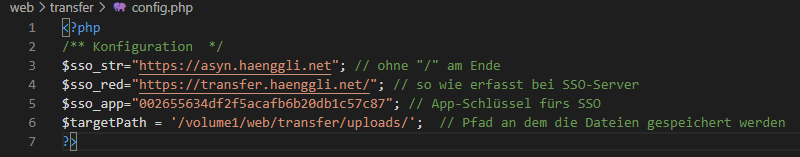
\includegraphics[width=1\linewidth]{content/images/prototyp_konfiguration.png}
    \caption{Konfigurationsmöglichkeiten des Prototyps}
    \label{fig:Konfigurationsmoeglichkeiten_prototyp}
\end{figure}
In den nächsten beiden Abschnitten werden die Gedanken zu den Konfigurationsmöglichkeiten erläutert.

\subsection{User Identifizierung}
Wie im Abschnitt \hyperref[subsec:Links]{Generierung der Links} beschrieben, dürfen Links fürs Hoch- und Herunterladen nur 
von Migratoren erstellt werden können. Dafür bedarf es eines Logins. Durch die vorgegebene Hardware ist es möglich, 
die bestehenden Benutzer des Synology NAS zu verwenden. Synology bietet eigens dafür eine Anleitung inkl. PHP- und Frontendbeispiele an \cite{Synology}.
Durch das so nutzbare Single Sign On entfällt eine zusätzliche Userverwaltung. 
So ist es einfach möglich Migratoren (=eingeloggte User) von Kunden (=nicht eingeloggte User) zu unterscheiden.
\\ 
Die nötigen Parameter für die Anbindung eins beliebigen Synology-NAS können mit den Variablen beginnend mit ``\$sso\_'' gesetzt werden.

\subsection{Datenhaltung}
Der ganze Prototyps verwaltet nur Dateien. Das ist eine Aufgabe, die das Dateisystem ebenfalls wahrnimmt.
Es ist daher sinnvoll, für die Haltung der Dateien auf das Dateisystem zurückzugreifen. 
Beim Prototyp muss daher nur angegeben werden, wo die Daten am Ende gespeichert werden sollen. 
Dies kann mit der Variable ``\$targetPath'' konfiguriert werden. 
Wird ein Pfad ausserhalb des eigentlichen WebServers hinterlegt, ist kein direkter Zugriff über eine URL auf eine Datei möglich.
Dies erhöht die Sicherheit und schützt die Daten vor unbefugten Zugriff aus dem Internet.

\section{Graphische Benutzeroberfläche}
Das Herzstück des Prototyps ist die Oberfläche. Diese entscheidet über gelingen oder nicht gelingen.
Wie in \cite{Butz} beschrieben, wird versucht eine möglichst einfache Oberfläche zu gestalten. Ohne verwirrende Farben oder Effekte.
Alle Links werden daher klassisch in blau gehalten. Alles andere sind nur Texte ohne dahinerliegende Aktionen.
Bei der ursprünglichen Recherche zu bestehenden Tools wurden von unzähligen Anbietern die JavaScript-Lösung DropzoneJs verwendet.
Diese frei verfügbare Bibliothek für die Oberfläche beinhaltet die clientseitig implementierte Lösung zu zahlreichen Hürden aus den Anforderungen:
Drag\&Drop von Dateien, 
Auswahl mittels Dialogbox, 
Statusanzeige über den Stand des Hochladens,
Rückmeldungen bei Erfolg und Fehler nach dem Hochladen,
Teilung von zu grossen Dateien, 
Anstoss um Teildateien serverseitig wieder zusammenzusetzen,
nach dem Zusammensetzen kann ein Log-Aufruf abgesetzt werden.

\clearpage
Die Dokumentation \cite{DropzoneJs} zu DropzoneJs ist sehr ausführlich und ebenfalls mit Serverseitigen PHP-Beispielen bestückt. 
Vermutlich einer der Gründe, wieso Tools wie Droppy oder YouTransfer darauf basieren.
Aufgrund der zahlreichen Vorteile und breiten Verwendung in Tools mit ähnlichen Möglichkeiten,
wird zur Implementation dieses Prototyps ebenfalls auf DropzoneJs zurückgegriffen.

\begin{figure}[!h]
    \centering
    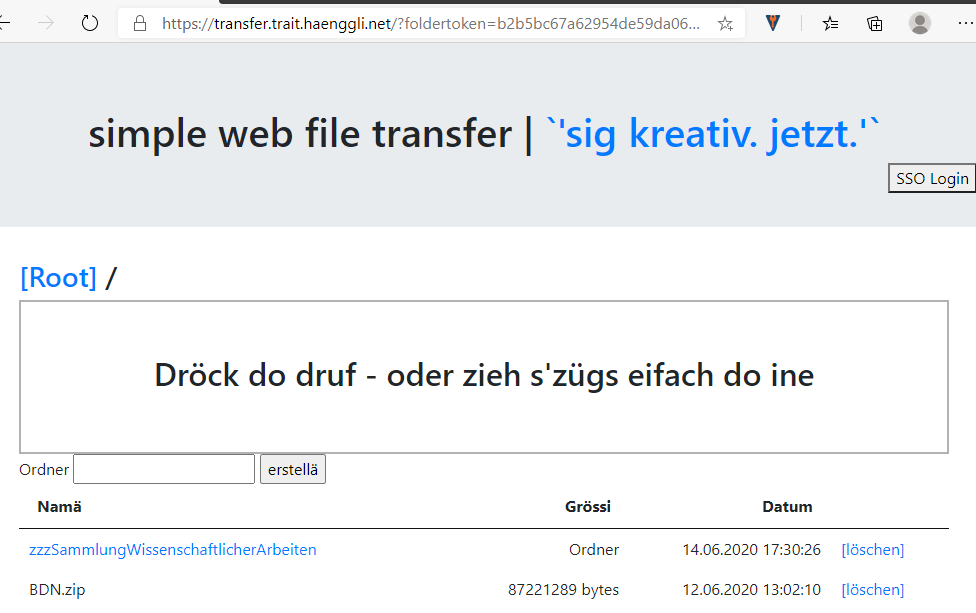
\includegraphics[width=1\linewidth]{content/images/prototyp_nichteingeloggt.png}
    \caption{Ansicht Prototyps von Kunde mittels Hochladelink}
    \label{fig:Prototyp_Hochladelink}
\end{figure} %\\
Wie in Abbildung \ref{fig:Prototyp_Hochladelink} ersichtlich, konnte die Oberfläche sehr einfach gehalten werden.
Hochladen und Löschen sind für Kunden möglich ohne die Daten wieder einzusehen. Für die bessere Strukturierung können unbeschränkt neue Unterordner erstellt werden.
Das Synology-Loginfenster kann mit Klick auf den Button ``SSO Login'' geöffnet werden. \\ 
    
\clearpage  

Einmal eingeloggt stehen weitere Möglichkeiten, sichtbar in Abbildung \ref{fig:Prototyp_Migrator}, zur Verfügung. 

\begin{figure}[!h]
    \centering
    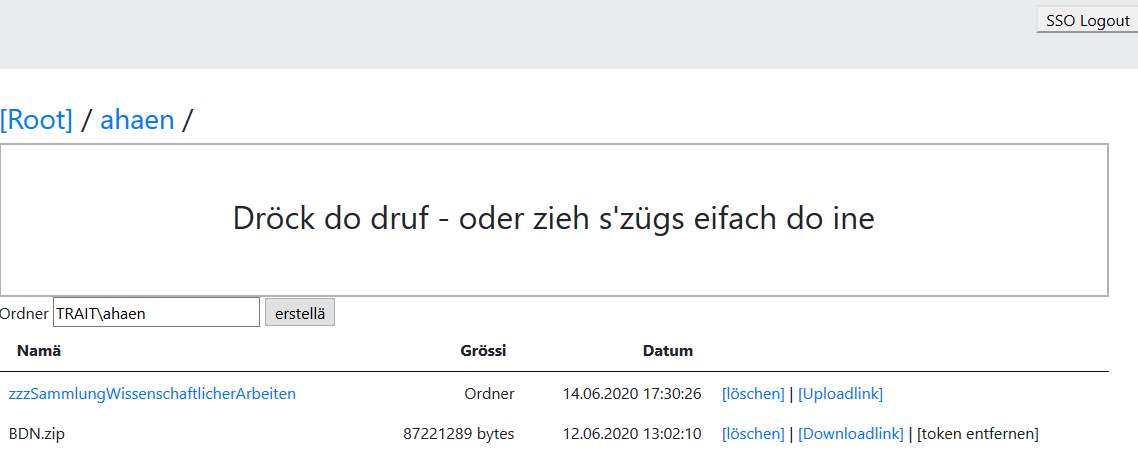
\includegraphics[width=1\linewidth]{content/images/prototyp_eingeloggt.png}
    \caption{Ansicht Prototyps nach Login}
    \label{fig:Prototyp_Migrator}
\end{figure}

Die zusätzlichen Möglichkeiten sind gemäss Abbildung \ref{fig:Prototyp_Migrator} 
die Ordnernavigation unabhängig vom Uploadlink, das erstellen weiterer Uploadlinks 
sowie das Erstellen von Downloadlinks.
Innerhalb des Netzwerk kann, wie in Abbildung \ref{fig:file_explorer} ersichtlich, mit dem üblichen Dateiexplorer auf alle Dateien und Ordner zugegriffen werden.

\begin{figure}[!h]
    \centering
    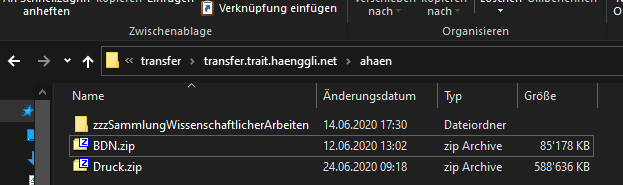
\includegraphics[width=1\linewidth]{content/images/file_explorer.png}
    \caption{Ansicht mit Dateiexplorer}
    \label{fig:file_explorer}
\end{figure}

%\clearpage
Die Nutzung eines Downloadlinks ist ebenso einfach. Er kann wie eine normale Website aufgerufen werden.
Der Browser bringt dann automatisch den jeweiligen Standard Download-Dialog. 
Ein Beispiel dazu findet sich mit Abbildung \ref{fig:ie_download}.
\begin{figure}[!h]
    \centering
    
\includegraphics[width=1\linewidth]{content/images/prototyp_download.png}
    \caption{Download-Dialog im Internet Explorer}
    \label{fig:ie_download}
\end{figure}

\section{Generierung von Links}
Um die Links fürs Hochladen und Herunterladen von Dateien nicht sprechend zu gestalten, werden zufällig generierte 32stellige Werte verwendet.
Diese können durch einen Aufruf der PHP\-Funktion ``random\_bytes(32)'' erzeugt werden.
Die so erzeugten Werte werden mit dem dazugehörenden Pfad abgespeichert. Als Pfad wird der Pfad zur Datei bei Download, 
sowie der Pfad zum Ordner fürs Hochladen verwendet.
Um erneut auf eine Datenbank zu verzichten, werden die Zuweisungen ebenfalls in einer PHP-Datei gespeichert.
Analog der Konfigurationsdatei kann die Datei mit den Zuweisungen zur Laufzeit geladen werden. So besteht für das Skript jederzeit Zugriff auf die Informationen.
Durch die PHP-Endung der Zuweisungsdatei ist der Inhalt nicht öffentlich aus dem Internet ersichtlich.
\\
Nicht eingeloggte User sind nicht in der Lage neue Links zu generieren. 
Eingeloggte User können mittels Knopfdruck - wie bei Abbildung \ref{fig:Prototyp_Migrator} ersichtlich - auf ``[Uploadlink]'' klicken. 
Serverseitig wird geprüft, ob es für den Ordner bereits einen zufälligen 32stelligen Wert gibt. Falls nicht, wird einer erstellt (Abbildung \ref{fig:Srv_newLink}):
\begin{figure}[!h]
    \centering
    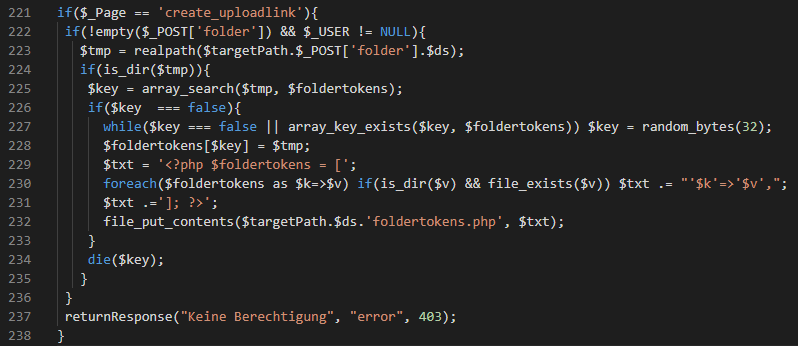
\includegraphics[width=0.9\linewidth]{content/images/prototyp_tokens.png}
    \caption{Serverseitige Generierung eines Links}
    \label{fig:Srv_newLink}
\end{figure}
  \\
Der so ermittelte Wert wird dann an die URL der Seite angehängt (siehe Abbildung \ref{fig:Hochladelink_prototyp}).
\begin{figure}[!h]
    \centering
    
\includegraphics[width=1\linewidth]{content/images/prototyp_uploadtoken.png}
    \caption{Neu generierter Hochladelink}
    \label{fig:Hochladelink_prototyp}
\end{figure}
  \\
Durch den Aufruf der Webseite mit dem URL-Parameter können die Kunden so nur die darin enthaltenen Dateien sehen. 
Ohne eine Möglichkeit diese herunterzuladen - wie bei Abbildung \ref{fig:Prototyp_Hochladelink} ersichtlich.

\section{Serverseitige Aufgaben}
Serverseitig mussten mit PHP folgende Aufgaben gelöst werden:
\begin{itemize}
    \item Kommunikation/Prüfung mit dem Synology-NAS zur Prüfung ob ein Benutzer eingeloggt ist gemäss \cite{Synology}
    \item Anbieten des Downloads bei gültigem Downloadlink
    \item Anzeige aller Ordner und Dateien anhand des Hochladelinks    
    \item Löschen von Dateien und Ordner falls ein gültiger Hochladelink verwendet wird (oder Benutzer eingeloggt ist)
    \item Loggen von hochgeladenen und heruntergeladenen Dateien für Analysezwecke
    \item Zusammensetzen von gesplitteten Dateien
    \item Falls eingeloggt: Anzeige ergänzen mit Möglichkeit Ordner zu wechseln
    \item Falls eingeloggt: Generierung von neuen Links für Hochladen und Herunterladen
\end{itemize}
\chapter{Analyse}
%\chapter{Analyse der Messungen}
\ToDo{Dokumentation der Ergebnisse}

\ToDo{Auswertung der Logfiles}
\ToDo{Performanz}
\ToDo{Feedback}
\chapter{Ausblick}
In Zukunft wird das in dieser Arbeit erstellte Konzept zu Testzwecken produktiv bei 100
IoT-Geräten eingesetzt. Die Evaluierung der Datenpunkte ist dabei noch nicht abgeschlossen
aber im Gange. Dabei werden die neuen Datenkorrelationen im Team diskutiert
und bewertet, die nach Abschluss dieses Verfahrens in die Firmware eingebaut
werden. Die Auswertung erfolgt dann in etwa drei Monaten nach der Aktualisierung. Dies
garantiert eine aussagekräftige Anzahl an Daten.
Um die Analysemöglichkeiten noch verbessern zu können, wird ausserdem MQTT als
neues Verbindungsprotokoll eingesetzt. Dieses Protokoll ermöglicht eine nahezu Realtime-
Analyse der gesammelten Daten, was eine geringere Reaktionszeit zur Folge hat. Diese
Strategie wird noch durch automatisierte Aktionen ergänzt, was den Arbeitsaufwand für
die Analyse minimal hält. Aus betrieblichen und datenschutzrechtlichen Gründen kann
die Strategie aber an dieser Stelle nicht näher ausgeführt werden.

\chapter{Reflexion}
Es handelt sich hierbei um meine erste wissenschaftliche Arbeit. 
Entsprechend musste ich mich vor Beginn stark in die Thematik einlesen. Dazu habe ich auch einige Beispielarbeiten gelesen.
Dies hat einiges an Zeit gekostet, wodurch ich mich viel zu spät damit auseinander gesetzt habe, 
über welches Thema ich schreiben soll. Das Coaching durch den Dozenten war daher sehr hilfreich. 
Während der Recherche zur dahinterliegenden Technologie der Arbeit, war es schwierig geeignete Quellen zu finden.
Die Themen werden in den Sachbüchern jeweils nur angeschnitten oder auf einem sehr hohen Expertenlevel sehr detailliert behandelt.
Das von mir gewünschte Mittelmass scheint leider nicht sehr weit verbreitet zu sein.
Dies kann an meiner Problemstellung zusammenliegen. Die zwar individuelle Lösung hat sehr allgemeingültige Grundlagen dahinter.
Netzwerke und deren Aufbau sind nicht gerade meine Stärke. 
Dennoch war es sehr interessant die Hintergründe dazu bei der Implementierung des Prototyps zu berücksichtigen.
\\
Ich bin froh darüber, dass es sich hierbei um eine erste wissenschaftliche Arbeit und keine Abschlussarbeit oder gar Bachelorarbeit handelt.
Mit den neu gewonnen Erfahrungen würde ich dort die Vorbereitungen und Recherche anders gestalten. 
Wäre mir von Beginn des Moduls an, ein Thema im Kopf gewesen, hätte ich die Arbeit wohl anders aufgebaut. 
Eine sinnvolle und möglichst vollständige Argumentation mit rotem Faden aufzubauen ist eine Herausforderung. 
Eventuell wäre es einfacher geworden, wenn die Fragestellung konkreter definiert worden wäre. 
Sie lässt eigentlich offen, ob der Prototyp nur ein Mittel zum Zweck oder aber der Entwurf dessen das Hauptziel ist. 
\\
Nichtsdestotrotz konnte an dieser Arbeit einiges an Erfahrung gewonnen werden. Mit den Resultaten bin ich im grossen und ganzen sehr zufrieden.
Bei der noch folgenden Bachelorarbeit werde ich jedoch die obigen Punkte verbessern. Besonders was die Definition der Fragestellung betrifft.



\listoffigures 

%\listoftables

%\begin{thebibliography}{XX}
%\bibitem[XY]{XY} blah
%\end{thebibliography}
% oder besser
% \bibliography{myBibTeXFile.bib}
\printbibliography

\newpage

\begin{appendix}


\chapter*{Selbstständigkeitserklärung}
Ich erkläre hiermit, dass ich diese Thesis selbständig verfasst 
und keine andern als die angegebenen Quellen benutzt habe. 
Alle Stellen, die wörtlich oder sinngemäss aus Quellen entnommen wurden, 
habe ich als solche kenntlich gemacht. Ich versichere zudem, dass ich bisher 
noch keine wissenschaftliche Arbeit mit gleichem oder ähnlichem Inhalt an der 
Fernfachhochschule Schweiz oder an einer anderen Hochschule eingereicht habe. 
Mir ist bekannt, dass andernfalls die Fernfachhochschule Schweiz zum Entzug 
des aufgrund dieser Thesis verliehenen Titels berechtigt ist.

\vspace{4cm}
\noindent
\hrule \ \\[-0.5ex]
Ort, Datum, Unterschrift



%\chapter*{Einverständniserklärung}
%Wir bestätigen hiermit, dass wir die vorstehende Arbeit (Module-Kürzel/Name) im Kollektiv 
%angefertigt haben und somit mit den abgelieferten Dokumenten einverstanden sind. 
%Im Sinne einer Gruppenarbeit akzeptieren wir eine kollektive 
%Bewertung unserer Arbeit.
%
%\vspace{2cm}
%\noindent
%\hrule \ \\[-0.5ex]
%Ort, Datum, Unterschrift


\end{appendix}

\end{document}


